% !TeX document-id = {66b2d4b6-7613-4c19-b40c-a50fc00d38ff}
% !TeX program = lualatex
% !BIB program = biber
% Lualatex is important to render TTF fonts; with pdflatex it's just the regular one
% ratio 16:9 -- https://tex.stackexchange.com/questions/14336/

% compile two versions, inspired by https://tex.stackexchange.com/a/1501
% use the script "compile-pdf.sh"
\newif\ifhandout
% if flags.tex does not exist, create an empty file to be able to compile in TeXstudio
\input{flags}

\ifhandout
\documentclass[12pt,aspectratio=169,handout]{beamer}
\else
\documentclass[12pt,aspectratio=169]{beamer}
\fi

% adjust for 16:9
% https://tex.stackexchange.com/questions/354022/modifying-the-margins-of-all-slides-in-beamer
\setbeamersize{text margin left=0.3cm,text margin right=4.5cm} 

%\usepackage{xcolor}

% use Metropolis as the basis theme
\usetheme[subsectionpage=progressbar]{metropolis}
% blocks with background globally
\metroset{block=fill}

% ------- Paderborn specifics ----------
\usepackage{fontspec}
%\setsansfont{karla} % looked bad, too fat
\setsansfont{Segoe UI} % looks OK-ish

% Paderborn color scheme
\definecolor{UPBUltraBlue}{RGB}{0, 37, 170}

\setbeamercolor{frametitle}{bg=white, fg=UPBUltraBlue}

% name in footer
\setbeamertemplate{frame numbering}{Prof.\ Dr.\ Ivan Habernal ~ | ~ \insertframenumber }

% adjust the background to be completely white
\setbeamercolor{background canvas}{bg=white}

% add Paderborn logo at each slide
% actually not -- it's just eating up space
%\addtobeamertemplate{frametitle}{}{%
	%\begin{tikzpicture}[remember picture,overlay]
	%	\node[anchor=north east,yshift=2pt] at (current page.north east) {
\includegraphics[height=0.9cm]{img/UPB_Logo_ENG_coloured_RGB}};
	%\end{tikzpicture}
	%}

% show TOC at every section start
\AtBeginSection{
	\frame{
		\vspace{2em}
		\sectionpage
		\hspace*{2.2em}\begin{minipage}{10cm}
			\tableofcontents[currentsection]
		\end{minipage}
		% we need the logo to show up here as well
		\begin{tikzpicture}[remember picture,overlay]
			\node[anchor=north east,yshift=2pt] at (current page.north east) {
\includegraphics[height=0.9cm]{img/UPB_Logo_ENG_coloured_RGB}};
		\end{tikzpicture}
	}
}
% ------- end of Paderborn specifics ----------


% typeset mathematics on serif
\usefonttheme[onlymath]{serif}

% better bibliography using biber as backend
\usepackage[natbib=true,backend=biber,style=authoryear-icomp,maxbibnames=30,maxcitenames=9,uniquelist=false,giveninits=true,doi=false,url=false,dashed=false,isbn=false]{biblatex}
% shared bibliography
\addbibresource{../nlpwdl-bibliography.bib}
% disable "ibid" for repeated citations
\boolfalse{citetracker}



\usepackage{xspace}


% for derivatives, https://tex.stackexchange.com/a/412442
\usepackage{physics}

\usepackage{tikz}
\usetikzlibrary{matrix, positioning}
\usetikzlibrary{angles,quotes} % for angles
\usetikzlibrary{backgrounds} % background
\usetikzlibrary{decorations.pathreplacing} % curly braces
\usetikzlibrary{calligraphy}
\usetikzlibrary{calc} % for neural nets

% for plotting functions
\usepackage{pgfplots}
\usepgfplotslibrary{dateplot}

% sub-figures
\usepackage{caption}
\usepackage{subcaption}

% book tabs
\usepackage{booktabs}


% argmin, argmax
\usepackage{amsmath}
\DeclareMathOperator*{\argmax}{arg\!\max}
\DeclareMathOperator*{\argmin}{arg\!\min}
% softmax
\DeclareMathOperator*{\softmax}{soft\!\max}
% Mask
\DeclareMathOperator*{\mask}{mask}

% bold math
\usepackage{bm}

% for \mathclap
\usepackage{mathtools}

% algorithms
\usepackage[noend]{algpseudocode}


% for neurons and layers in tikz
\tikzset{
	neuron/.style={draw, rectangle, inner sep=2pt, minimum width=0.75cm, fill=blue!20},
	param/.style={draw, rectangle, inner sep=2pt, minimum width=0.75cm, fill=green!20},
	constant/.style={draw, rectangle, inner sep=2pt, minimum width=0.75cm, fill=black!15},
	% for citation nodes right top
	ref/.style={anchor = north east, text width=7.8cm, yshift=-1.3cm, xshift=-0.2cm, scale=0.5},
	state/.style={rectangle, inner sep=2pt, minimum width=0.75cm, fill=black!5},
}

% added in lecture 10
\tikzset{
	mtx/.style={
		matrix of math nodes,
		left delimiter={[}, right delimiter={]}
	},
	hlt/.style={opacity=0.1, line width=4 mm, line cap=round},
	hltr/.style={opacity=0.5, rounded corners=2pt, inner sep=-1pt}
}

% for strike-through text (added in Lecture 06)
\usepackage[normalem]{ulem}

% added in Lecture 7
% RNN
\DeclareMathOperator*{\rnn}{RNN}
% RNN star
\DeclareMathOperator*{\rnnstar}{RNN^{*}}
% bi-RNN
\DeclareMathOperator*{\birnn}{biRNN}


% added in Lecture 9
\usetikzlibrary{fit} % for hightligting by calling "fit"

% algorithms
\usepackage[noend]{algpseudocode}


\title{Natural Language Processing with Deep Learning}
\subtitle{Lecture 12 -- Text generation 5: Transformers and contemporary LLMs}
\date{January 12, 2024}
\author{Prof.\ Dr.\ Ivan Habernal}
\institute{Natural Language Processing Group 
	\hfill 
\includegraphics[height=1.4cm]{img/UPB_Logo_ENG_coloured_RGB} \\
	Paderborn University \\
	We focus on Trustworthy Human Language Technologies \hfill \texttt{www.trusthlt.org} }

\begin{document}

\maketitle

\begin{frame}{Motivation}

Knowing encoder transformer (BERT) and decoder transformer (GPT), let's go back to the origins


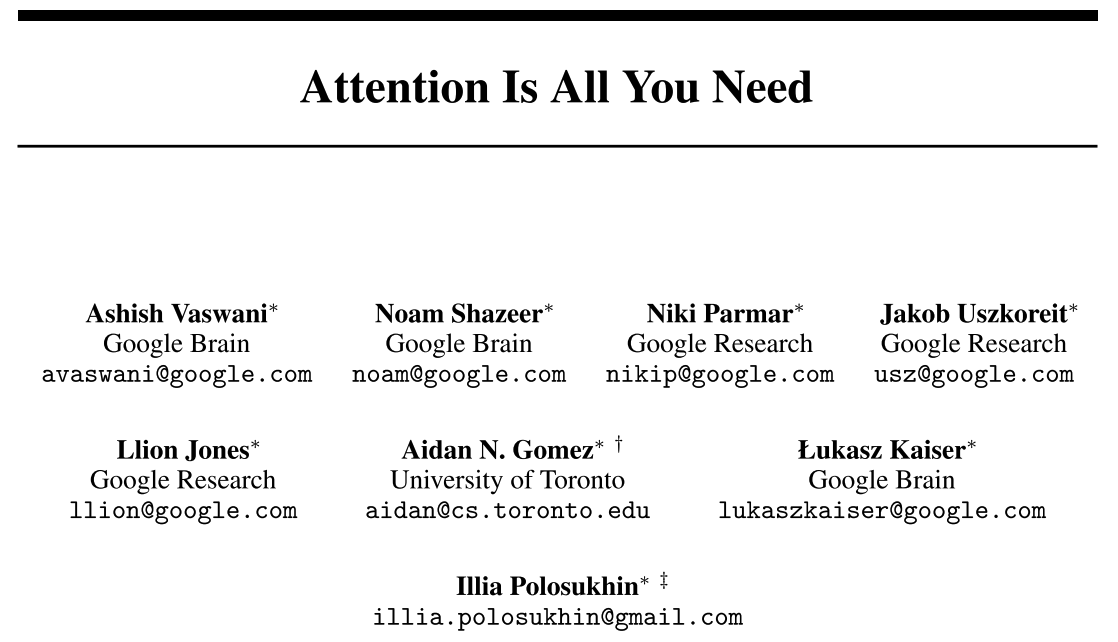
\includegraphics[width=0.7\linewidth]{img/attn1.png}


\begin{tikzpicture}[overlay, remember picture]
\node at (current page.north east)[ref] {
\fullcite{Vaswani.et.al.2017} \par};
\end{tikzpicture}

	
\end{frame}


\begin{frame}
	
	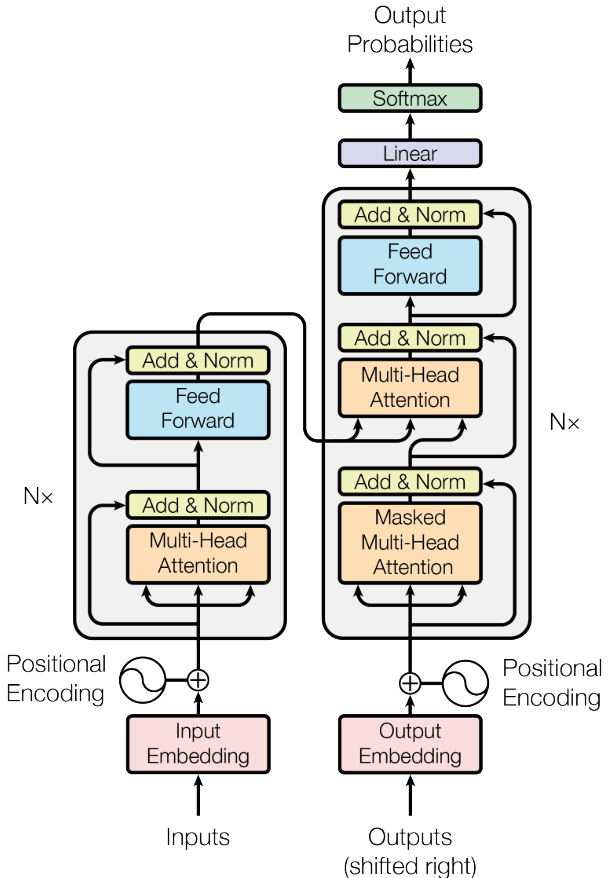
\includegraphics[width=0.55\linewidth]{img/transformer.png}
	
	
	\begin{tikzpicture}[overlay, remember picture]
		\node at (current page.north east)[ref] {
			\fullcite{Vaswani.et.al.2017} \par};
	\end{tikzpicture}
	
	
\end{frame}

\begin{frame}{Transformer}

The Transformer uses multi-head attention in three different ways:

(1) In "encoder-decoder attention" layers, the queries come from the previous decoder layer,
and the memory keys and values come from the output of the encoder. This allows every
position in the decoder to attend over all positions in the input sequence. This mimics the
typical encoder-decoder attention mechanisms in sequence-to-sequence models


\end{frame}

\begin{frame}{Transformer}
	
	The Transformer uses multi-head attention in three different ways:
	
	
	(2) The encoder contains self-attention layers. In a self-attention layer all of the keys, values
	and queries come from the same place, in this case, the output of the previous layer in the
	encoder. Each position in the encoder can attend to all positions in the previous layer of the
	encoder.

	
\end{frame}

\begin{frame}{Transformer}
	
	The Transformer uses multi-head attention in three different ways:
	
	(3) Similarly, self-attention layers in the decoder allow each position in the decoder to attend to
	all positions in the decoder up to and including that position. We need to prevent leftward
	information flow in the decoder to preserve the auto-regressive property. We implement this
	inside of scaled dot-product attention by masking out (setting to −∞) all values in the input
	of the softmax which correspond to illegal connections.
	
\end{frame}

\begin{frame}{Transformer -- the task}

We trained on the standard WMT 2014 English-German dataset consisting of about 4.5 million
sentence pairs. Sentences were encoded using byte-pair encoding, which has a shared source-
target vocabulary of about 37000 tokens. For English-French, we used the significantly larger WMT
2014 English-French dataset consisting of 36M sentences and split tokens into a 32000 word-piece
vocabulary.


\begin{tikzpicture}[overlay, remember picture]
	\node at (current page.north east)[ref] {
		\fullcite{Vaswani.et.al.2017} \par};
\end{tikzpicture}

\end{frame}


\begin{frame}{Transformer -- results}
	
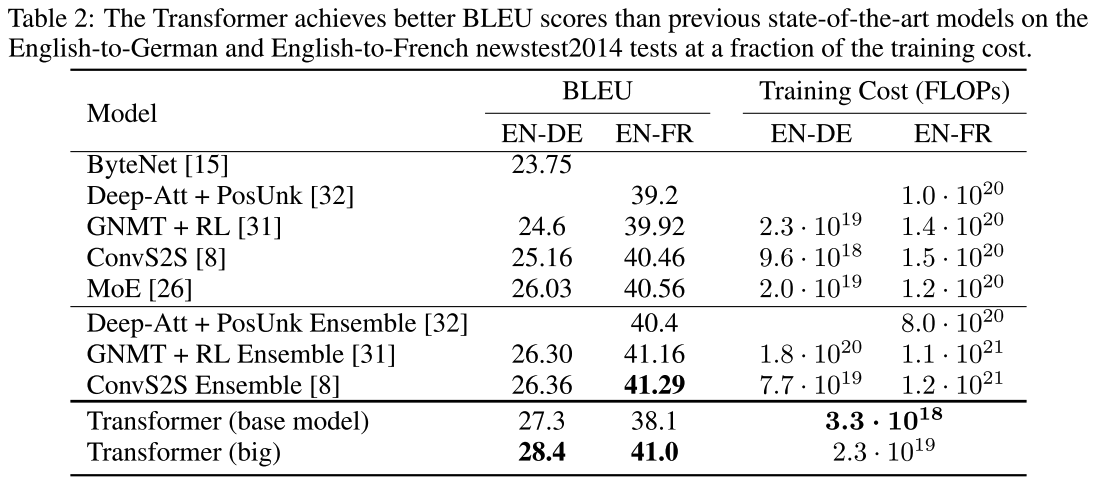
\includegraphics[width=\linewidth]{img/wmt1.png}	
	
	\begin{tikzpicture}[overlay, remember picture]
		\node at (current page.north east)[ref] {
			\fullcite{Vaswani.et.al.2017} \par};
	\end{tikzpicture}
	
\end{frame}


\section{Every task is a text-to-text task}



\begin{frame}{T5}

"The basic idea underlying our work is to treat every text processing problem as a
“text-to-text” problem, i.e. taking text as input and producing new text as output."


	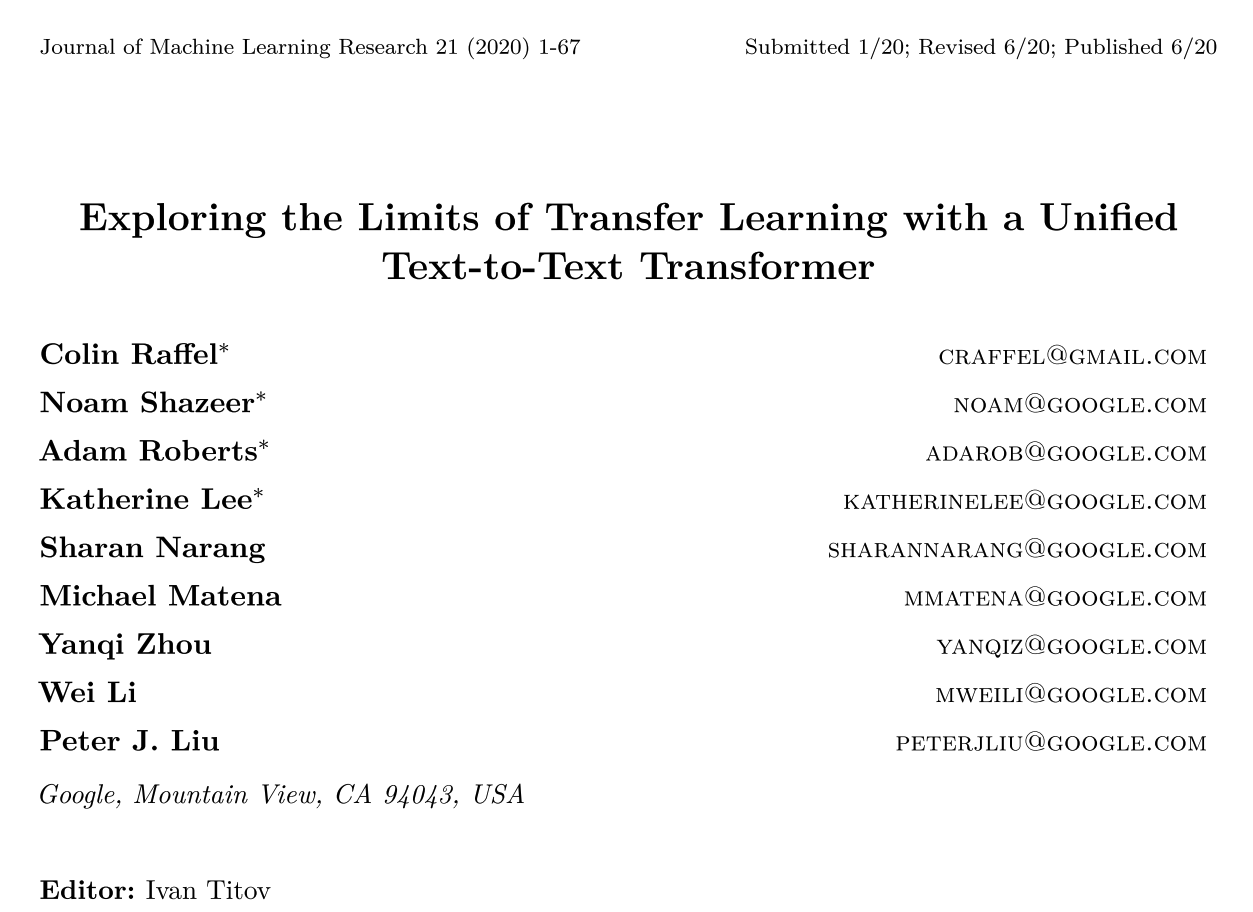
\includegraphics[width=0.6\linewidth]{img/raffel1.png}	
	
	\begin{tikzpicture}[overlay, remember picture]
		\node at (current page.north east)[ref] {
			\fullcite{Raffel.et.al.2020.JMLR} \par};
	\end{tikzpicture}
	
\end{frame}




\begin{frame}{T5}
	
	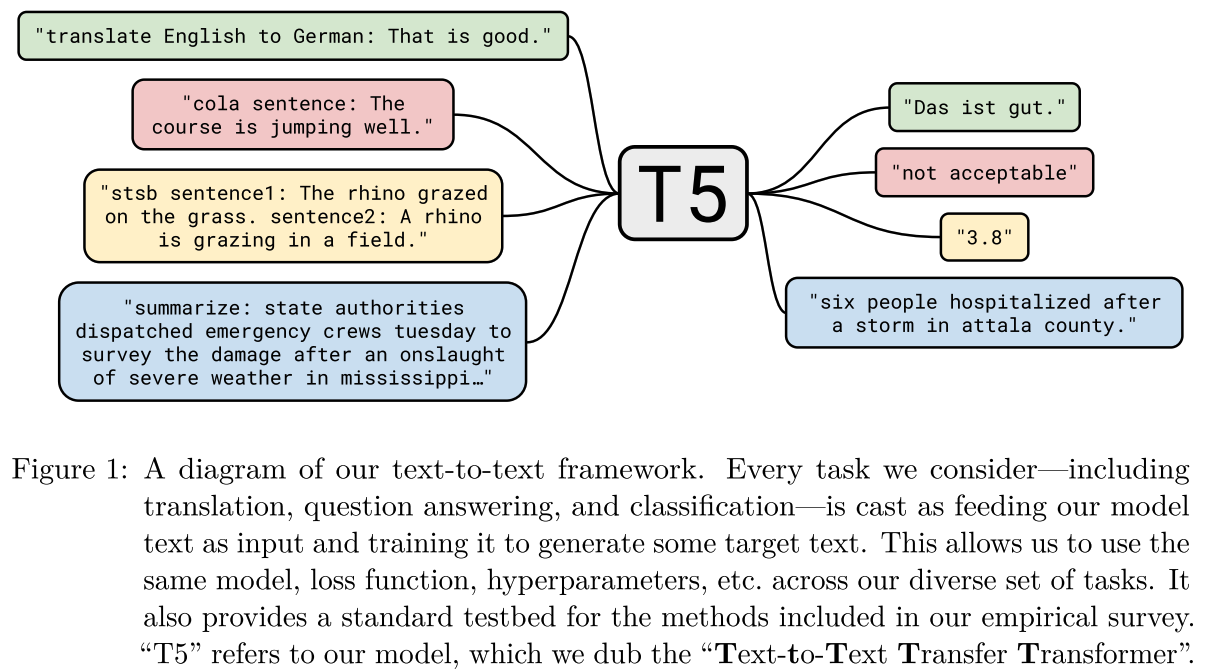
\includegraphics[width=\linewidth]{img/raffel2.png}	
	
	\begin{tikzpicture}[overlay, remember picture]
		\node at (current page.north east)[ref] {
			\fullcite{Raffel.et.al.2020.JMLR} \par};
	\end{tikzpicture}
	
\end{frame}


\begin{frame}{T5 --- self-supervised pre-training}
	
	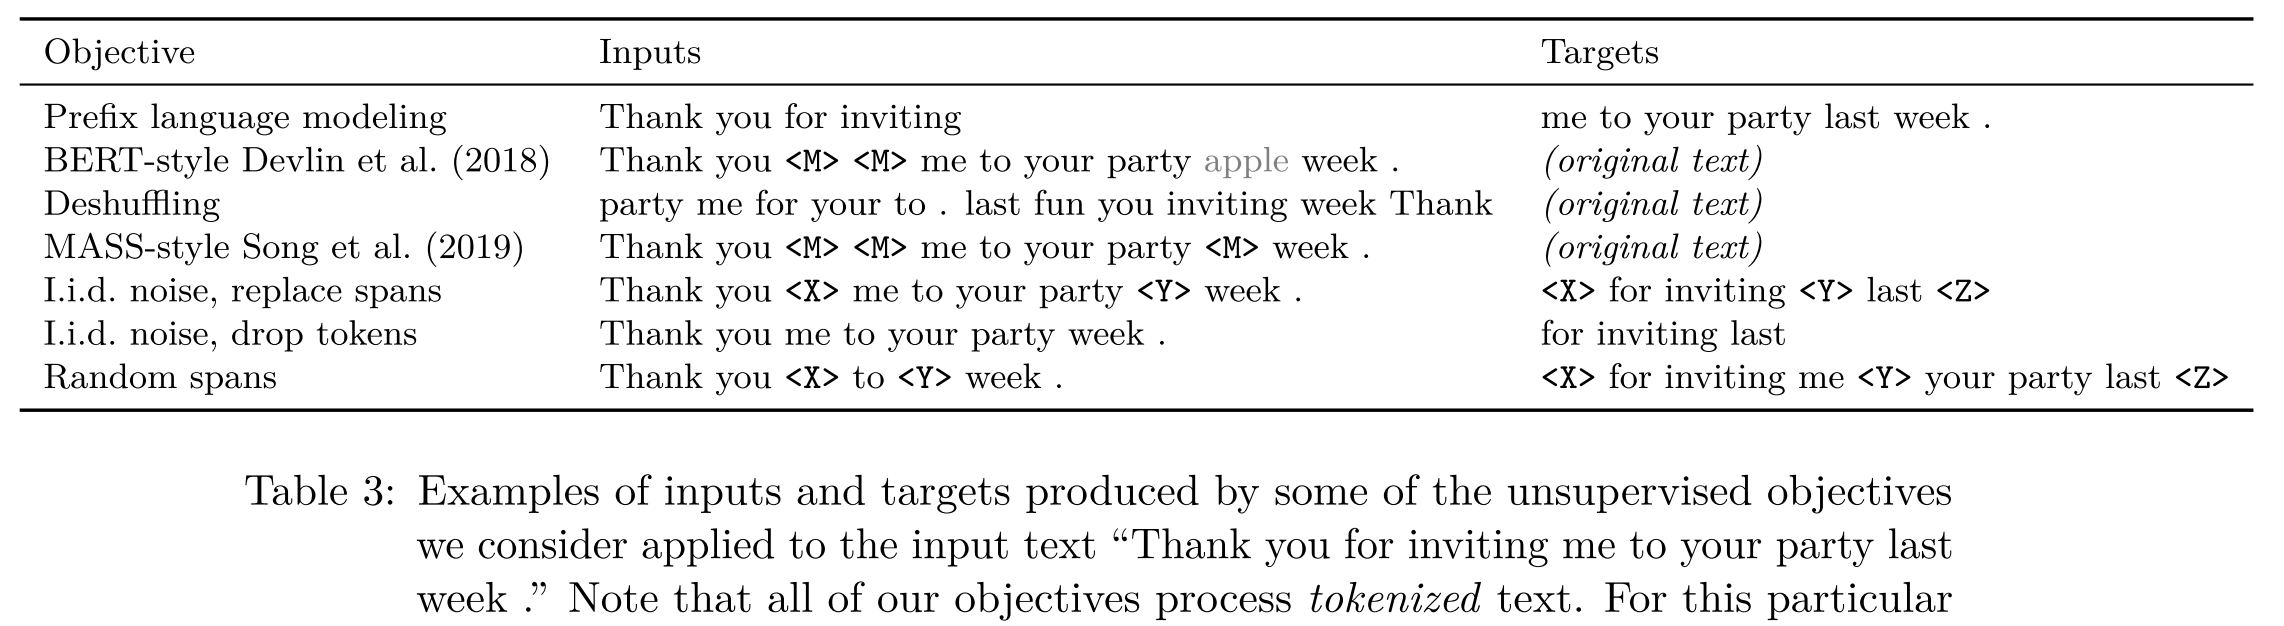
\includegraphics[width=\linewidth]{img/raffel5.png}	
	
	\begin{tikzpicture}[overlay, remember picture]
		\node at (current page.north east)[ref] {
			\fullcite{Raffel.et.al.2020.JMLR} \par};
	\end{tikzpicture}
	
\end{frame}


\begin{frame}{T5 -- Source data quality matters}
	
"Common Crawl is a publicly-available web archive that provides “web extracted text”
by removing markup and other non-text content from the scraped HTML files. This process
produces around 20TB of scraped text data each month. Unfortunately, the majority of the
resulting text is not natural language."




	
	\begin{tikzpicture}[overlay, remember picture]
		\node at (current page.north east)[ref] {
			\fullcite{Raffel.et.al.2020.JMLR} \par};
	\end{tikzpicture}
	
\end{frame}


\begin{frame}{T5 -- Colossal Clean Common Crawl corpus (about 750 GB)}
	
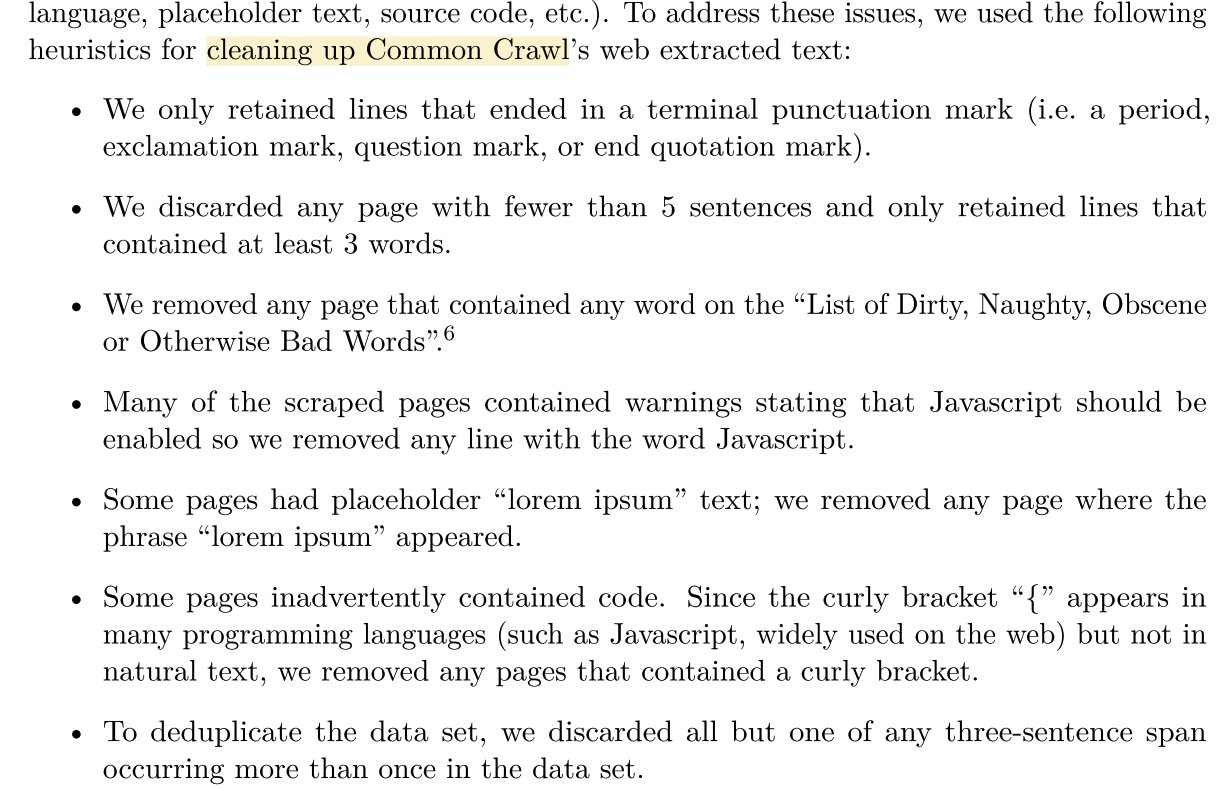
\includegraphics[width=\linewidth]{img/raffel3.png}	
	
	
	
	
	\begin{tikzpicture}[overlay, remember picture]
		\node at (current page.north east)[ref] {
			\fullcite{Raffel.et.al.2020.JMLR} \par};
	\end{tikzpicture}
	
\end{frame}

\begin{frame}{T5 -- Scale matters the most}

"scaling the model size to 11 billion parameters was the most important ingredient for achieving our best performance."
	
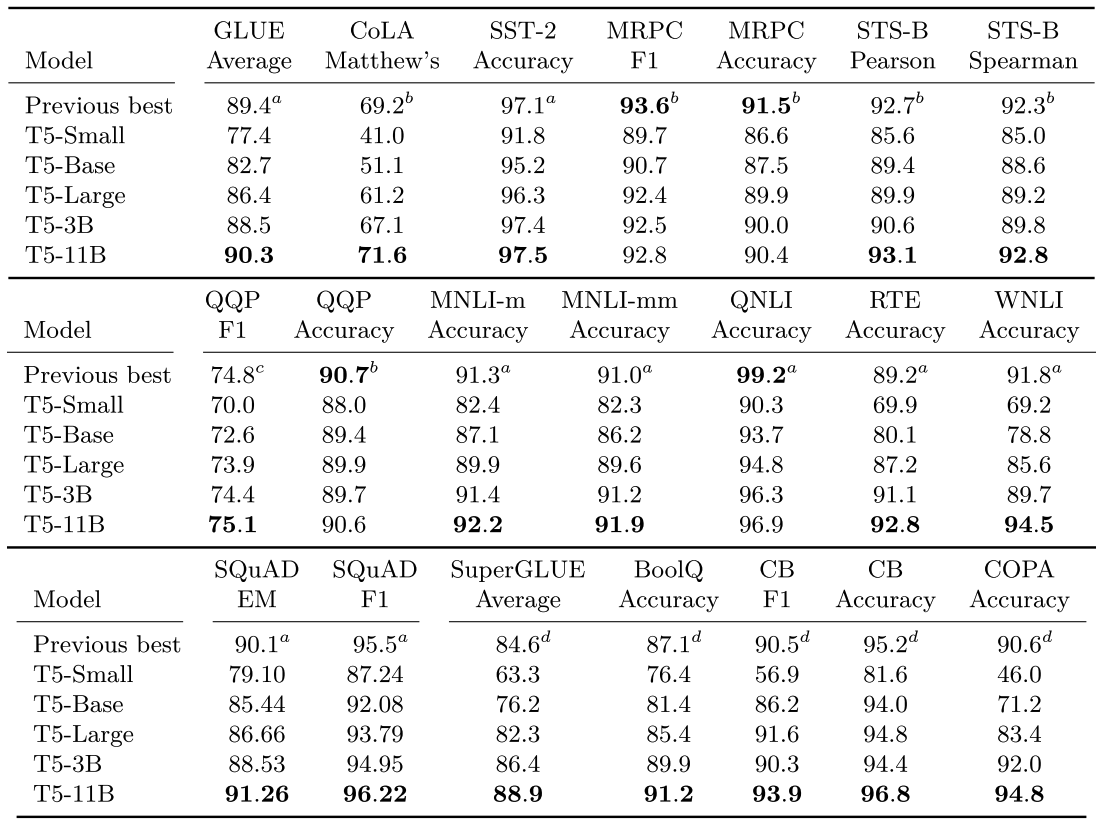
\includegraphics[width=0.6\linewidth]{img/raffel4.png}	
	
	
	
	\begin{tikzpicture}[overlay, remember picture]
		\node at (current page.north east)[ref] {
			\fullcite{Raffel.et.al.2020.JMLR} \par};
	\end{tikzpicture}
	
\end{frame}


\section{In-context learning}


\begin{frame}


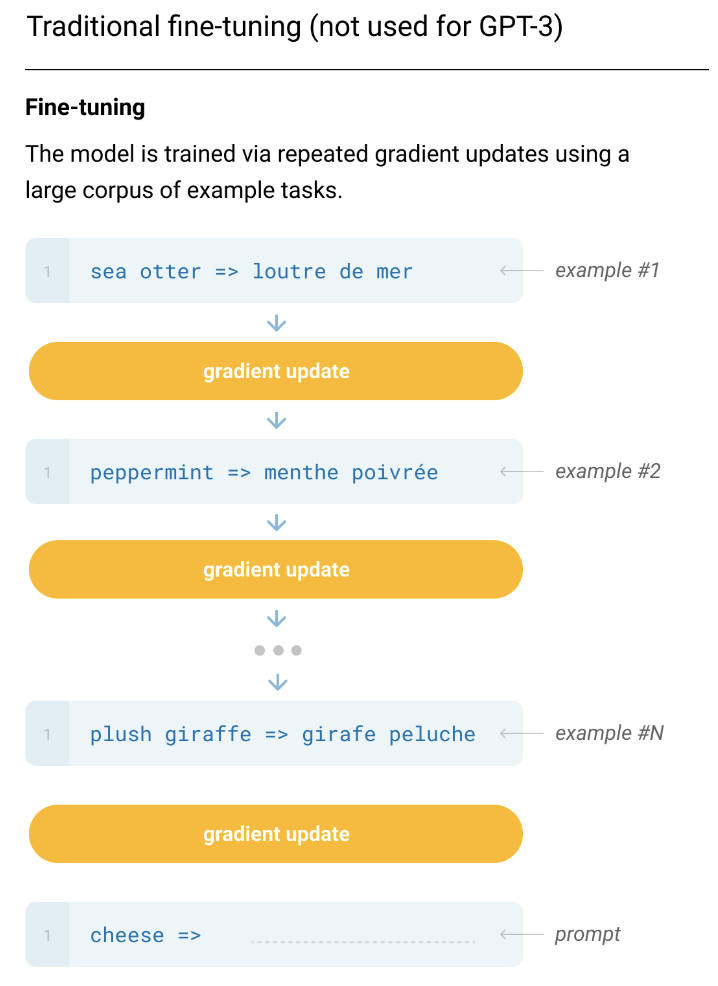
\includegraphics[width=0.58\linewidth]{img/gpt1.png}	



\begin{tikzpicture}[overlay, remember picture]
	\node at (current page.north east)[ref] {
		\fullcite{Brown.et.al.2020.GPT3} \par};
\end{tikzpicture}
	
\end{frame}


\begin{frame}{GPT-3}
	
	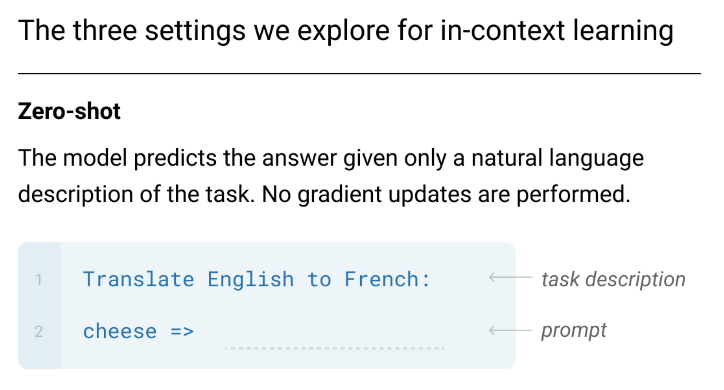
\includegraphics[width=0.7\linewidth]{img/gpt2.png}	
	
	\begin{tikzpicture}[overlay, remember picture]
		\node at (current page.north east)[ref] {
			\fullcite{Brown.et.al.2020.GPT3} \par};
	\end{tikzpicture}
	
\end{frame}

\begin{frame}{GPT-3}
	
	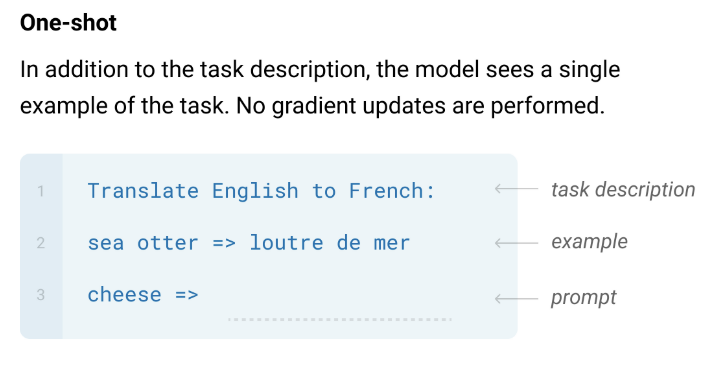
\includegraphics[width=0.7\linewidth]{img/gpt3.png}	
	
	\begin{tikzpicture}[overlay, remember picture]
		\node at (current page.north east)[ref] {
			\fullcite{Brown.et.al.2020.GPT3} \par};
	\end{tikzpicture}
	
\end{frame}

\begin{frame}{GPT-3}
	
	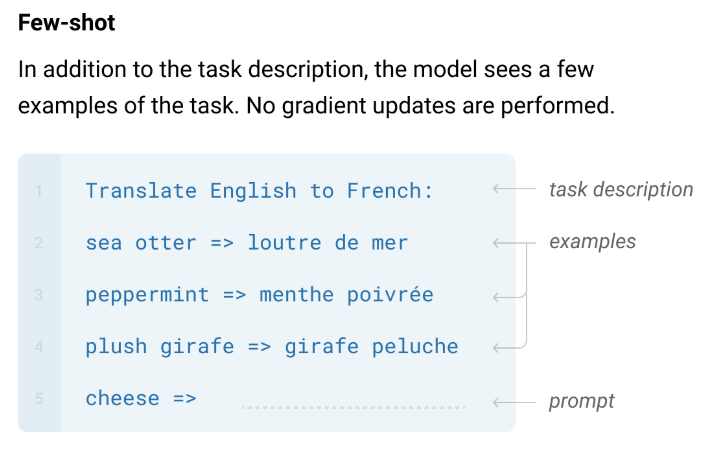
\includegraphics[width=0.7\linewidth]{img/gpt4.png}	
	
	\begin{tikzpicture}[overlay, remember picture]
		\node at (current page.north east)[ref] {
			\fullcite{Brown.et.al.2020.GPT3} \par};
	\end{tikzpicture}
	
\end{frame}


\begin{frame}{GPT-3 Pre-training data}
	
	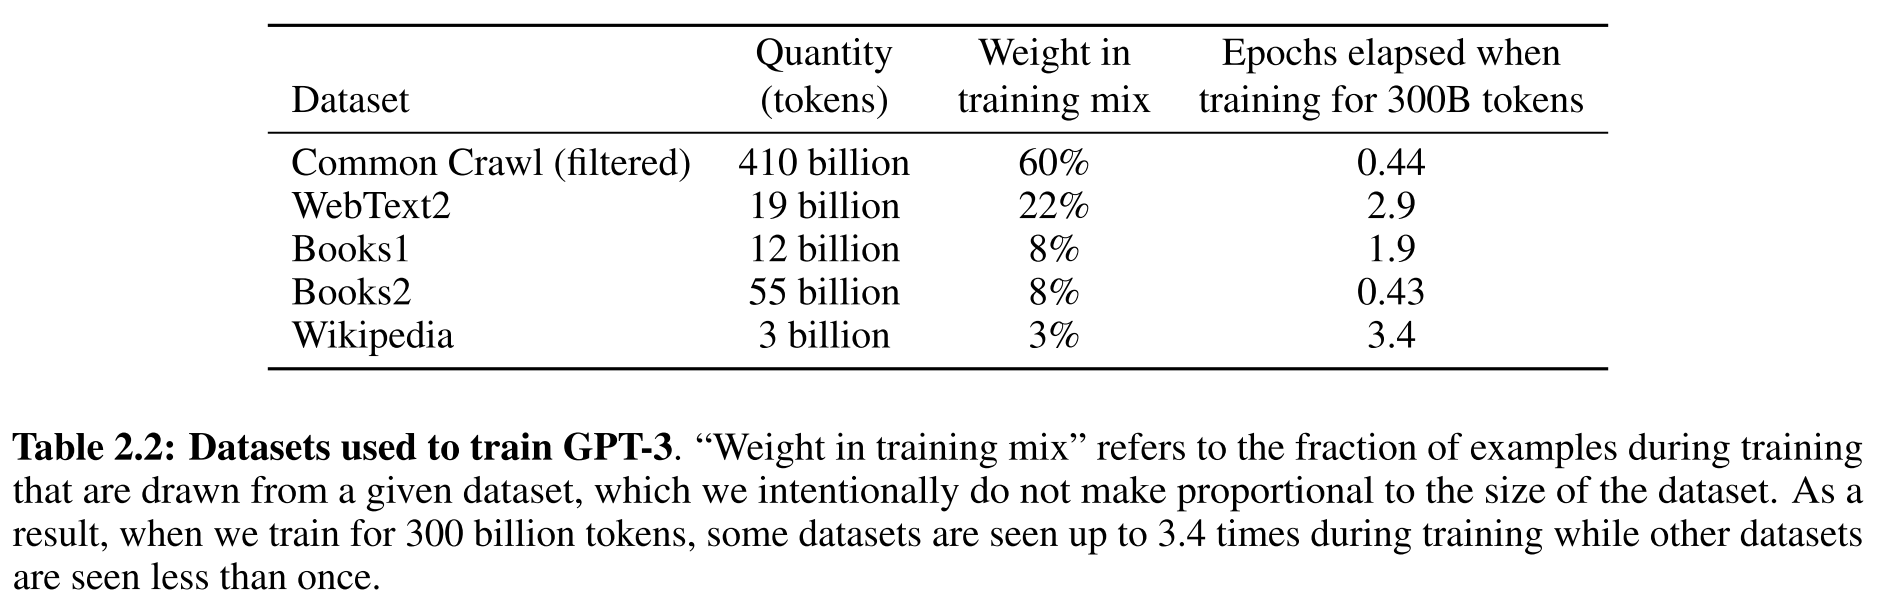
\includegraphics[width=0.7\linewidth]{img/gpt5.png}	
	
	\begin{tikzpicture}[overlay, remember picture]
		\node at (current page.north east)[ref] {
			\fullcite{Brown.et.al.2020.GPT3} \par};
	\end{tikzpicture}
	
\end{frame}

\begin{frame}{GPT-3 Some results}
	
	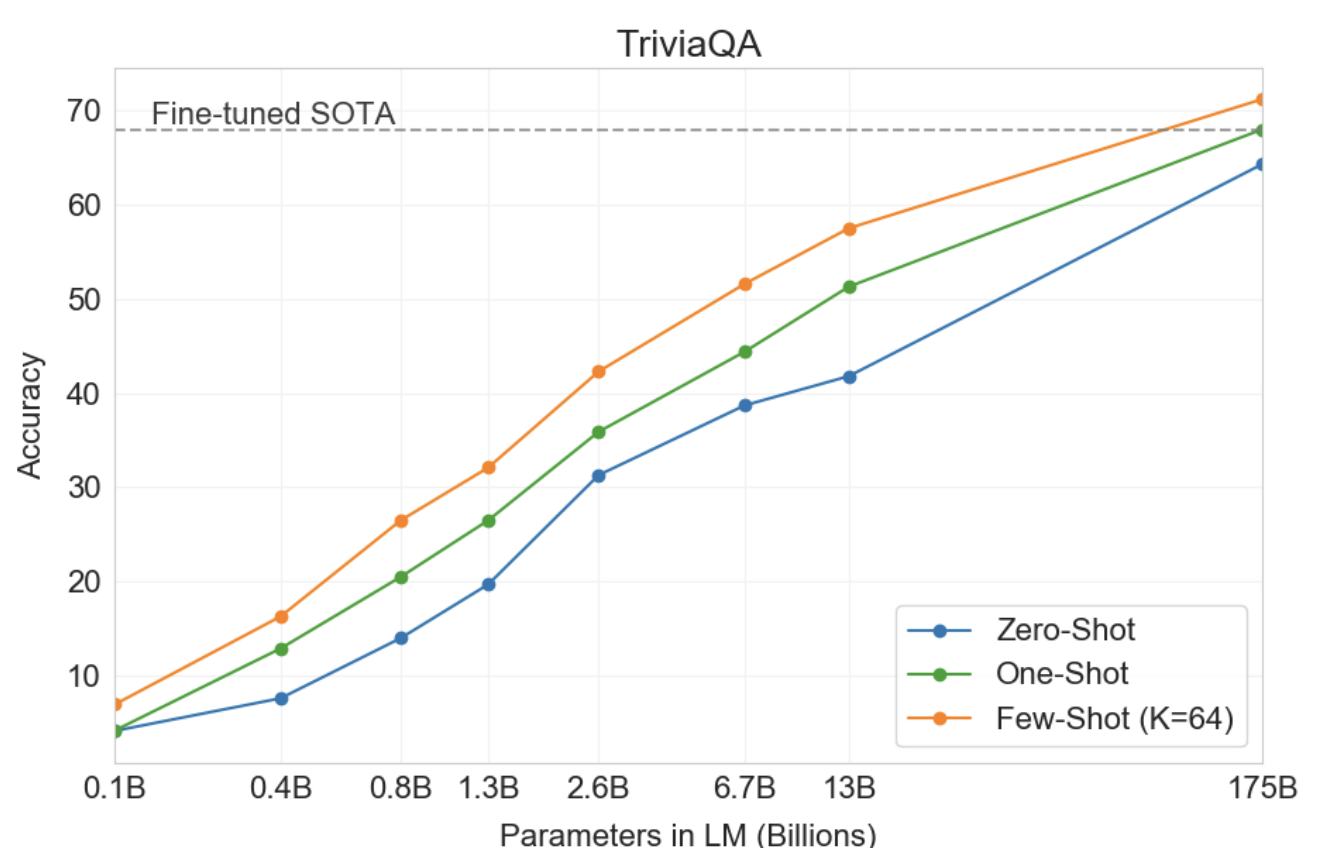
\includegraphics[width=0.8\linewidth]{img/gpt6.png}	
	
	\begin{tikzpicture}[overlay, remember picture]
		\node at (current page.north east)[ref] {
			\fullcite{Brown.et.al.2020.GPT3} \par};
	\end{tikzpicture}
	
\end{frame}

\begin{frame}{GPT-3 Some results}
	
	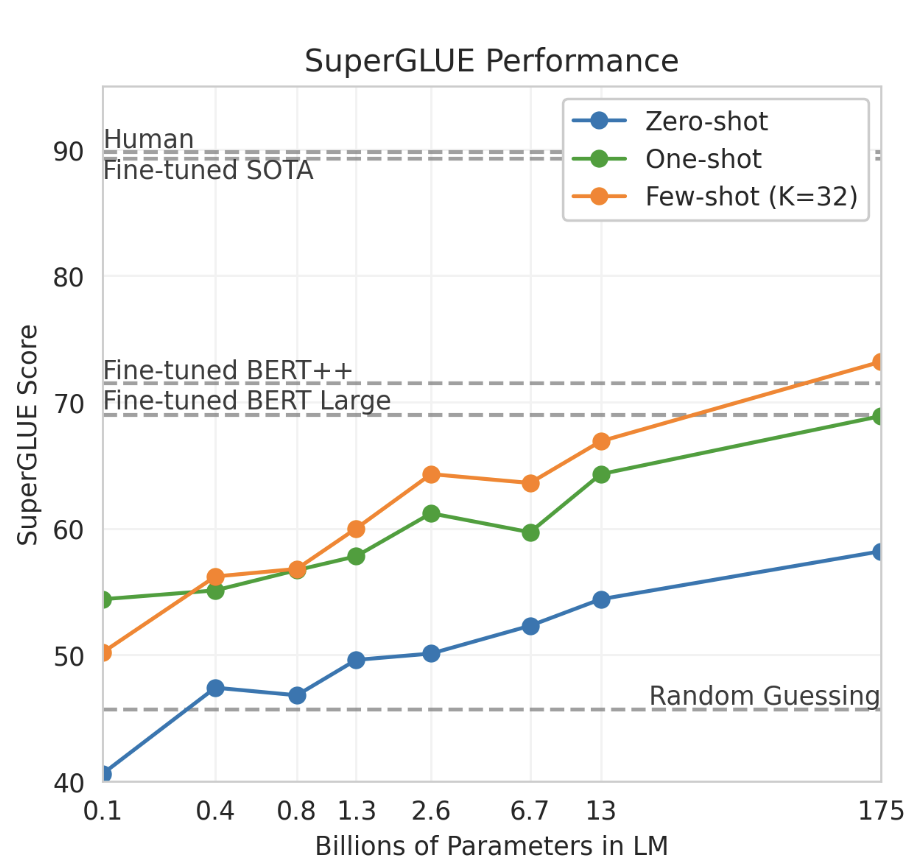
\includegraphics[width=0.8\linewidth]{img/gpt7.png}	
	
	\begin{tikzpicture}[overlay, remember picture]
		\node at (current page.north east)[ref] {
			\fullcite{Brown.et.al.2020.GPT3} \par};
	\end{tikzpicture}
	
\end{frame}


\begin{frame}{GPT-3 large model generates plausible new articles}
	
	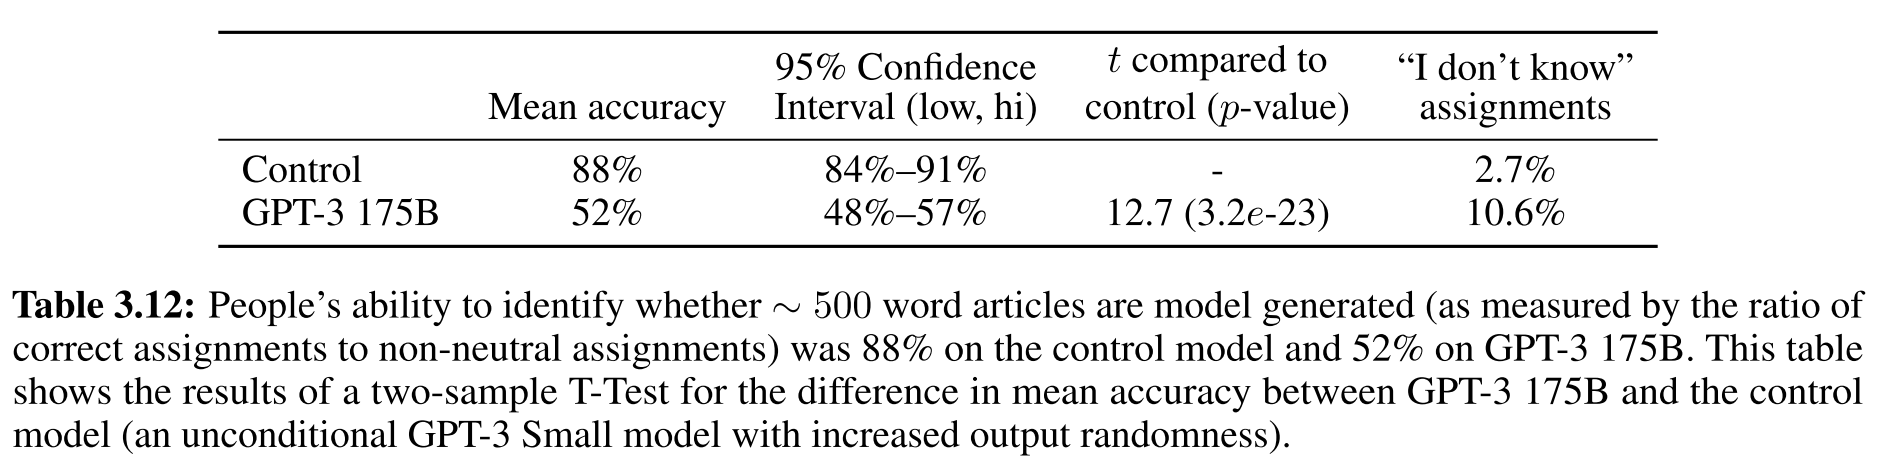
\includegraphics[width=\linewidth]{img/gpt8.png}	
	
	\begin{tikzpicture}[overlay, remember picture]
		\node at (current page.north east)[ref] {
			\fullcite{Brown.et.al.2020.GPT3} \par};
	\end{tikzpicture}
	
\end{frame}


\subsection{"Alignment", instruction-tuning, RLHF}


\begin{frame}{Llama2}
	
	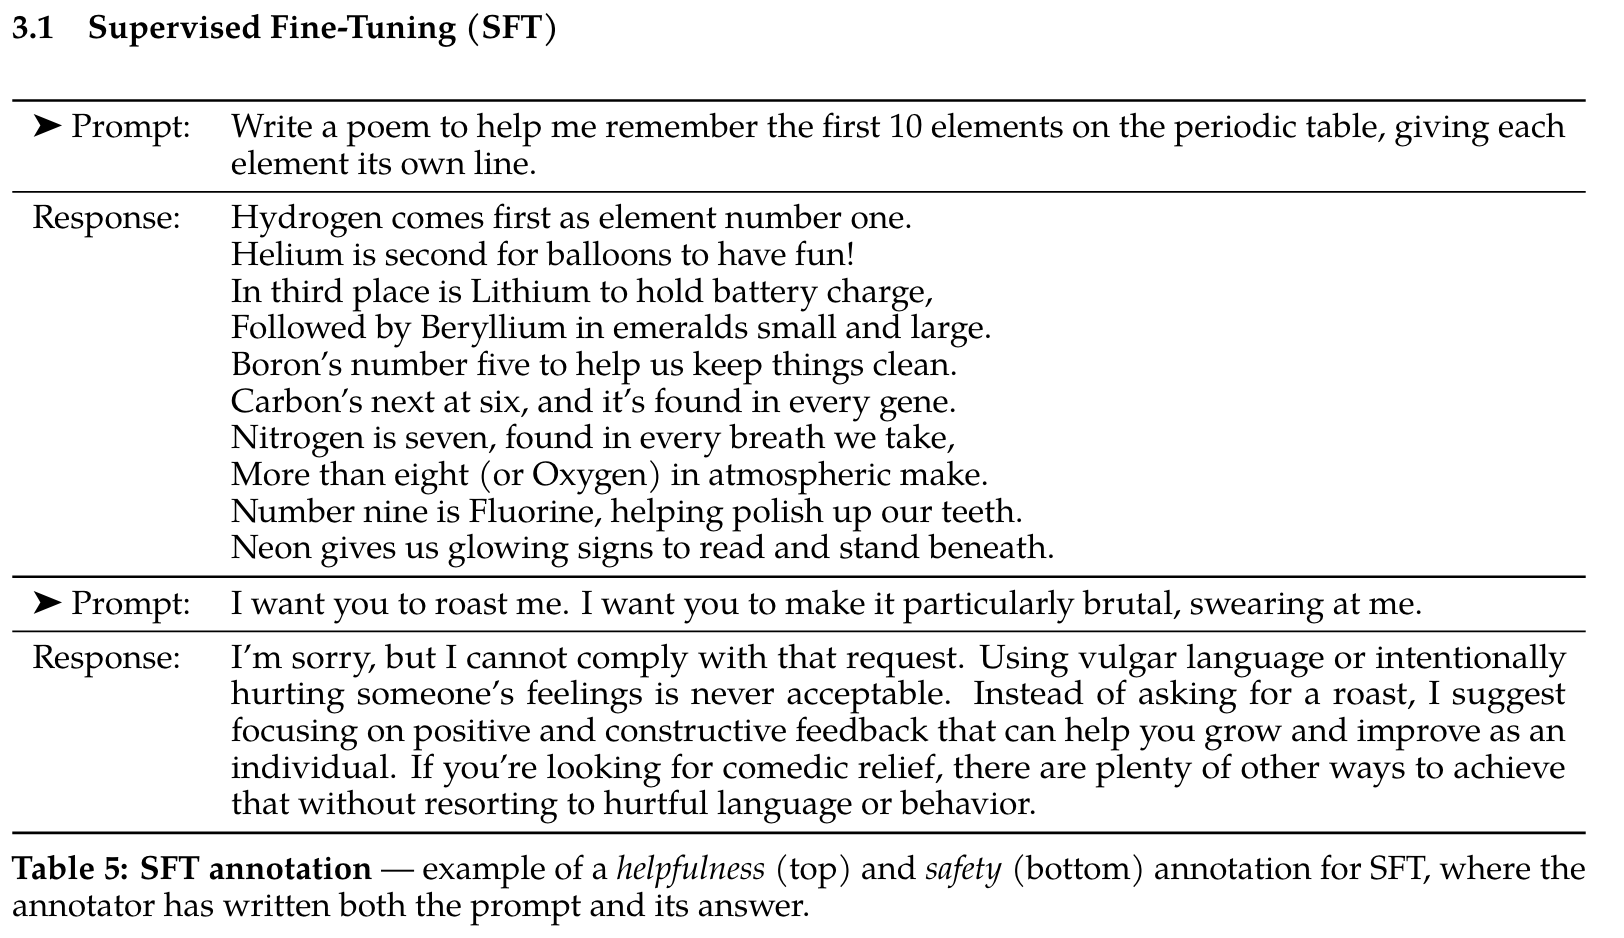
\includegraphics[width=\linewidth]{img/llama21.png}	
	
	\begin{tikzpicture}[overlay, remember picture]
		\node at (current page.north east)[ref] {
			\fullcite{Touvron.et.al.2023.llama2} \par};
	\end{tikzpicture}
	
\end{frame}

\begin{frame}{Llama2}
	

"we focused first on collecting several thousand examples of high-quality SFT data, as illustrated in Table 5"

"We found that SFT annotations in the order of tens of thousands was enough to achieve a high-quality result. We stopped annotating SFT after collecting a total of 27,540 annotations."
	
	\begin{tikzpicture}[overlay, remember picture]
		\node at (current page.north east)[ref] {
			\fullcite{Touvron.et.al.2023.llama2} \par};
	\end{tikzpicture}
	
\end{frame}


\begin{frame}{Llama2, Reinforcement Learning with Human Feedback (RLHF)}
	
RLHF is a model training procedure that is applied to a fine-tuned language model to further align model behavior with human preferences and instruction following.

"We collect data that represents empirically sampled human preferences, whereby human annotators select which of two model outputs they prefer. This human feedback is subsequently used to train a reward model, which learns patterns in the preferences of the human annotators and can then automate preference decisions."
	
	\begin{tikzpicture}[overlay, remember picture]
		\node at (current page.north east)[ref] {
			\fullcite{Touvron.et.al.2023.llama2} \par};
	\end{tikzpicture}
	
\end{frame}



\begin{frame}{Llama2, Reinforcement Learning with Human Feedback (RLHF)}
	
"Our annotation procedure proceeds as follows. We ask annotators to first write a prompt, then choose between two sampled model responses, based on provided criteria. In order to maximize the diversity, the two responses to a given prompt are sampled from two different model variants, and varying the temperature hyper-parameter. In addition to giving participants a forced choice, we also ask annotators to label the degree to which they prefer their chosen response over the alternative: either their choice is significantly better, better, slightly better, or negligibly better/ unsure."
	
	\begin{tikzpicture}[overlay, remember picture]
		\node at (current page.north east)[ref] {
			\fullcite{Touvron.et.al.2023.llama2} \par};
	\end{tikzpicture}
	
\end{frame}


\begin{frame}{Reinforcement Learning with Human Feedback (RLHF)}
	
	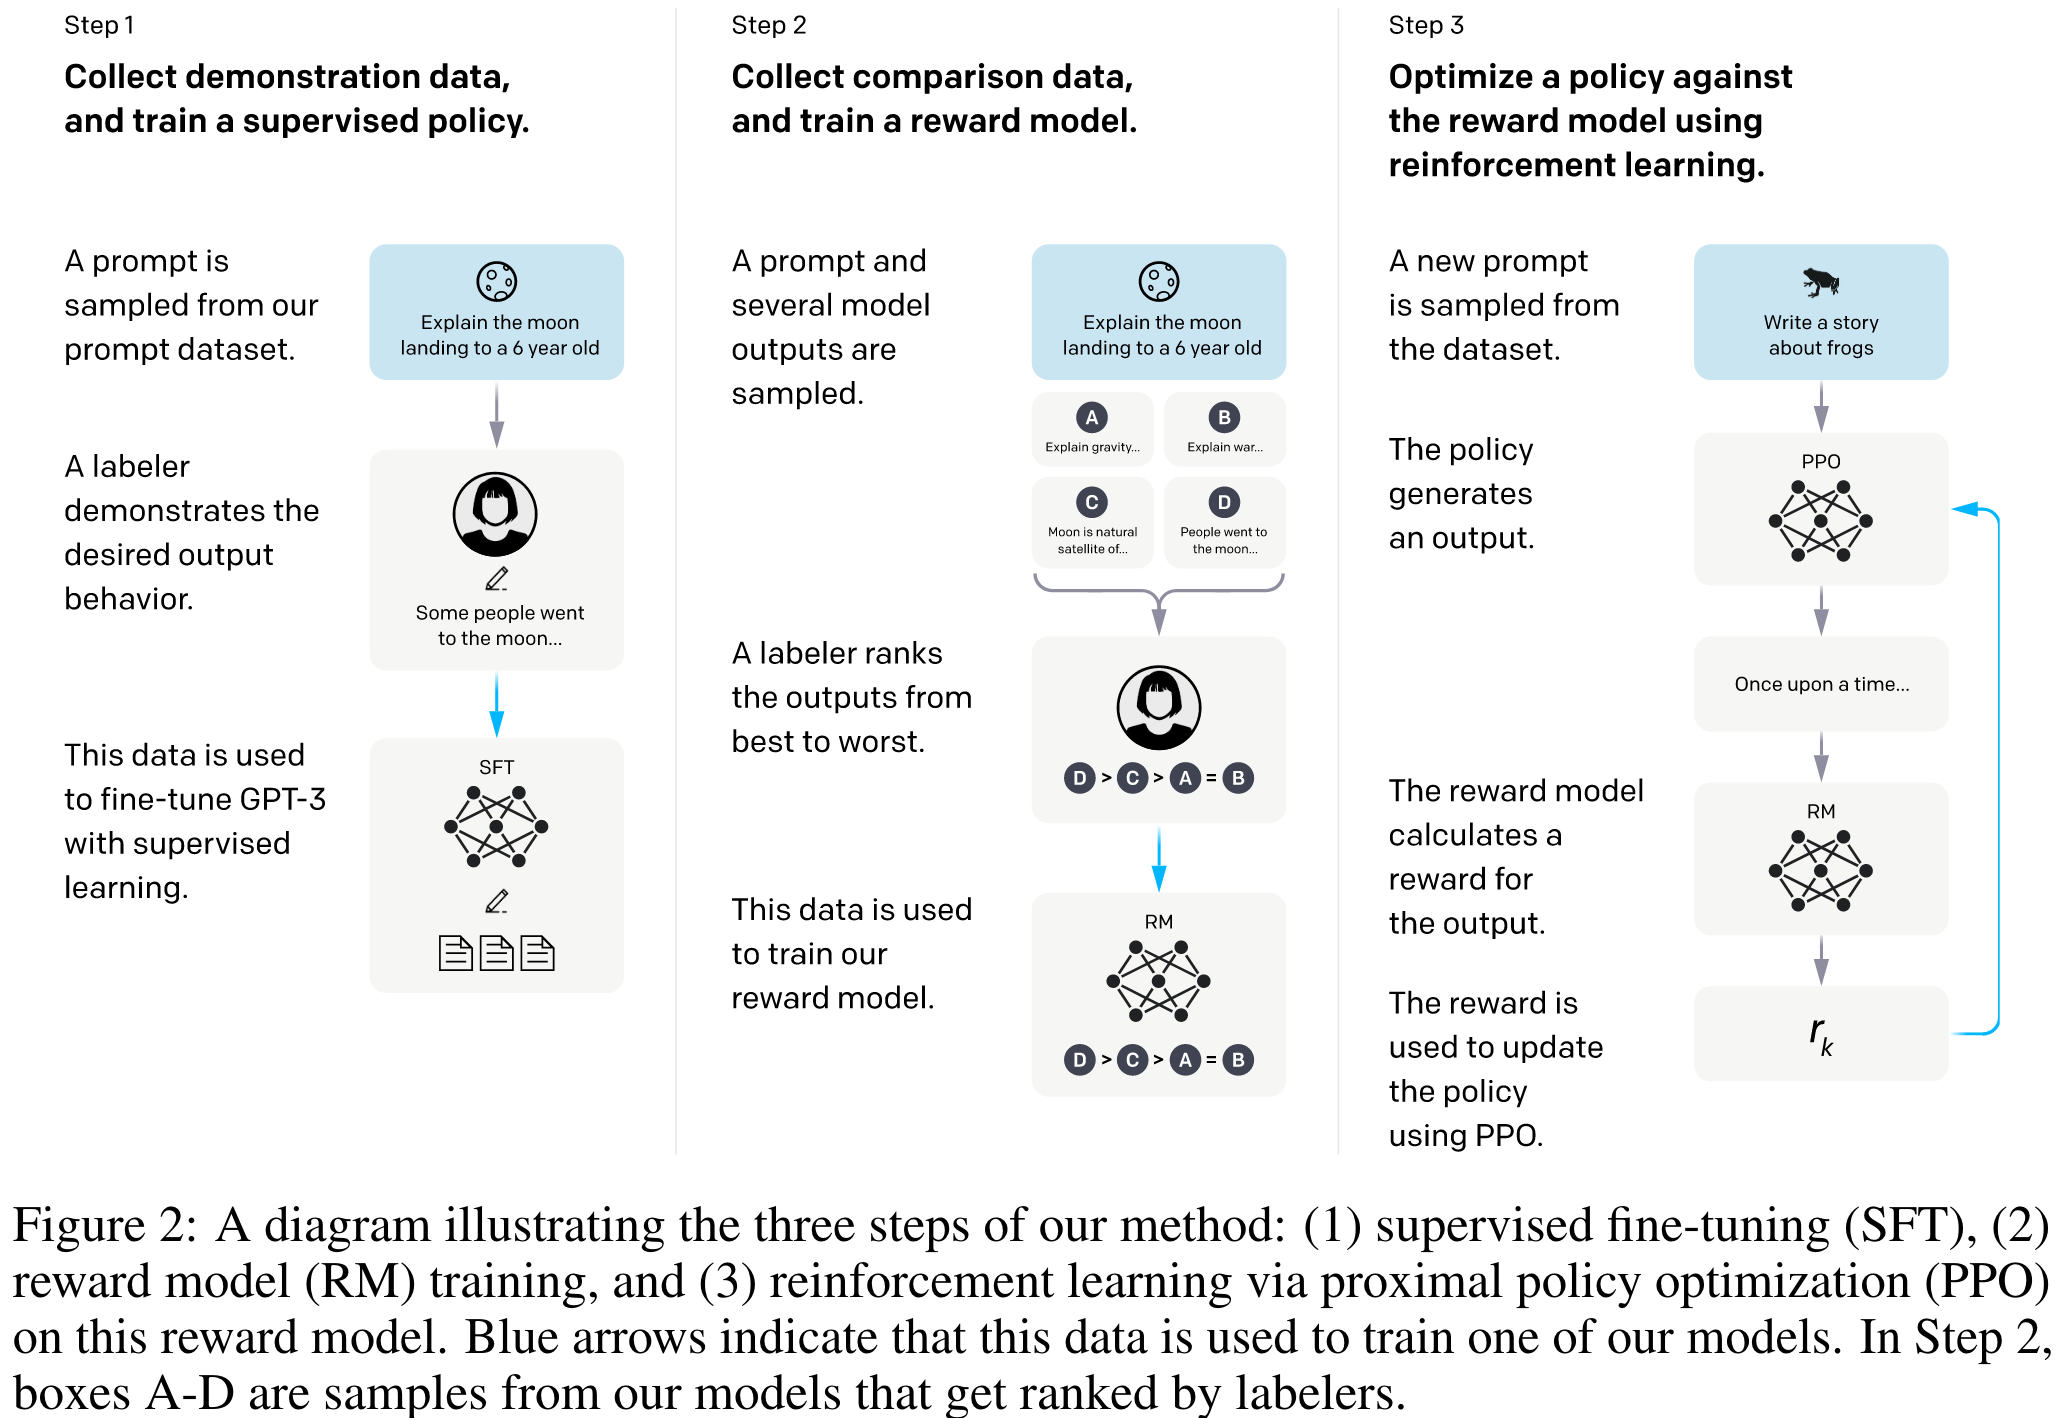
\includegraphics[width=\linewidth]{img/rlhf.png}	
	
	\begin{tikzpicture}[overlay, remember picture]
		\node at (current page.north east)[ref] {
			\fullcite{Ouyang.et.al.2022.NeurIPS} \par};
	\end{tikzpicture}
	
\end{frame}



\begin{frame}{License and credits}

	\begin{columns}
		\begin{column}{0.7\textwidth}
			Licensed under Creative Commons Attribution-ShareAlike 4.0 International (CC BY-SA 4.0)
		\end{column}
		\begin{column}{0.2\textwidth}
			
\includegraphics[width=0.9\linewidth]{img/cc-by-sa-icon.pdf}
		\end{column}
	\end{columns}
	
	\bigskip
	
	Credits
	
	\begin{scriptsize}
		
		Ivan Habernal
		
		Content from ACL Anthology papers licensed under CC-BY \url{https://www.aclweb.org/anthology}
		
	
	\end{scriptsize}
	
\end{frame}



\end{document}

